\section{Results}
\label{sec:results}
% =============================================================================

\subsection{Quantitative overview and scope}
\label{subsec:results_overview}

Table~\ref{tab:global_model_comparison} places the reported experiments at the beginning of the chapter. The FNO, standalone CVAE, and latent propagators solve different tasks, so their errors must not be ranked across blocks. Within the latent-propagator block, all models use the same pairwise representation and held-out test trajectories. A dash denotes a quantity that was not retained under a sufficiently controlled protocol; it is not a value of zero.

\begin{table}[H]
    \centering
    \small
    \caption{Overview of the models evaluated in this work. The standalone CVAE is a snapshot-reconstruction model. The Transformer and GNO rows compare propagation on the common test set. FNO metrics were not exported under the final common protocol and are therefore treated qualitatively.}
    \label{tab:global_model_comparison}
    \begin{tabular}{llrrrrr}
        \toprule
        Task & Model & $\epsilon_{\mathrm{rel}}$ & $SW$ & Moment error & $B_H$ & $t_{\mathrm{inf}}$ [ms] \\
        \midrule
        Longitudinal & FNO & -- & -- & -- & -- & -- \\
        Snapshot & CVAE & 0.367 & 0.0096 & 0.264 & -- & -- \\
        \midrule
        Propagation & Transformer, global & 0.681 & 0.087 & 9.838 & 17.337 & 18.74 \\
        Propagation & Transformer, $W=1$ & 0.650 & 0.026 & 63.047 & 52.389 & 14.35 \\
        Propagation & Transformer, $W=8$ & 0.534 & \textbf{0.014} & 56.169 & 50.414 & 12.01 \\
        Propagation & CVAE--GNO & \textbf{0.511} & 0.022 & \textbf{0.547} & \textbf{0.376} & \textbf{2.338} \\
        \bottomrule
    \end{tabular}
\end{table}

The table exhibits a Pareto trade-off rather than one model winning every metric. The $W=8$ Transformer has the lowest sliced-Wasserstein discrepancy, whereas the GNO has the lowest relative histogram error, moment error, residual-bias norm, and inference time. Inference timing compares neural models only; Chapter~\ref{sec:simulation_workflow} explains why no controlled simulator speed-up is claimed. The table reports selected checkpoints and does not include variation over repeated training seeds.

\subsection{Longitudinal operator learning with FNO}
\label{subsec:results_fno}

The preliminary longitudinal block evaluates the reduced map
\begin{equation}
    \widehat{\mathcal{T}}_{\theta}:
    (\lambda_{\mathrm{in}},\mu)
    \longmapsto
    \widehat{\lambda}_{\mathrm{out}}.
    \label{eq:fno_longitudinal_map_results}
\end{equation}
The task provides a controlled demonstration of density-to-density operator learning before the higher-dimensional latent study.

\begin{figure}[H]
    \centering
    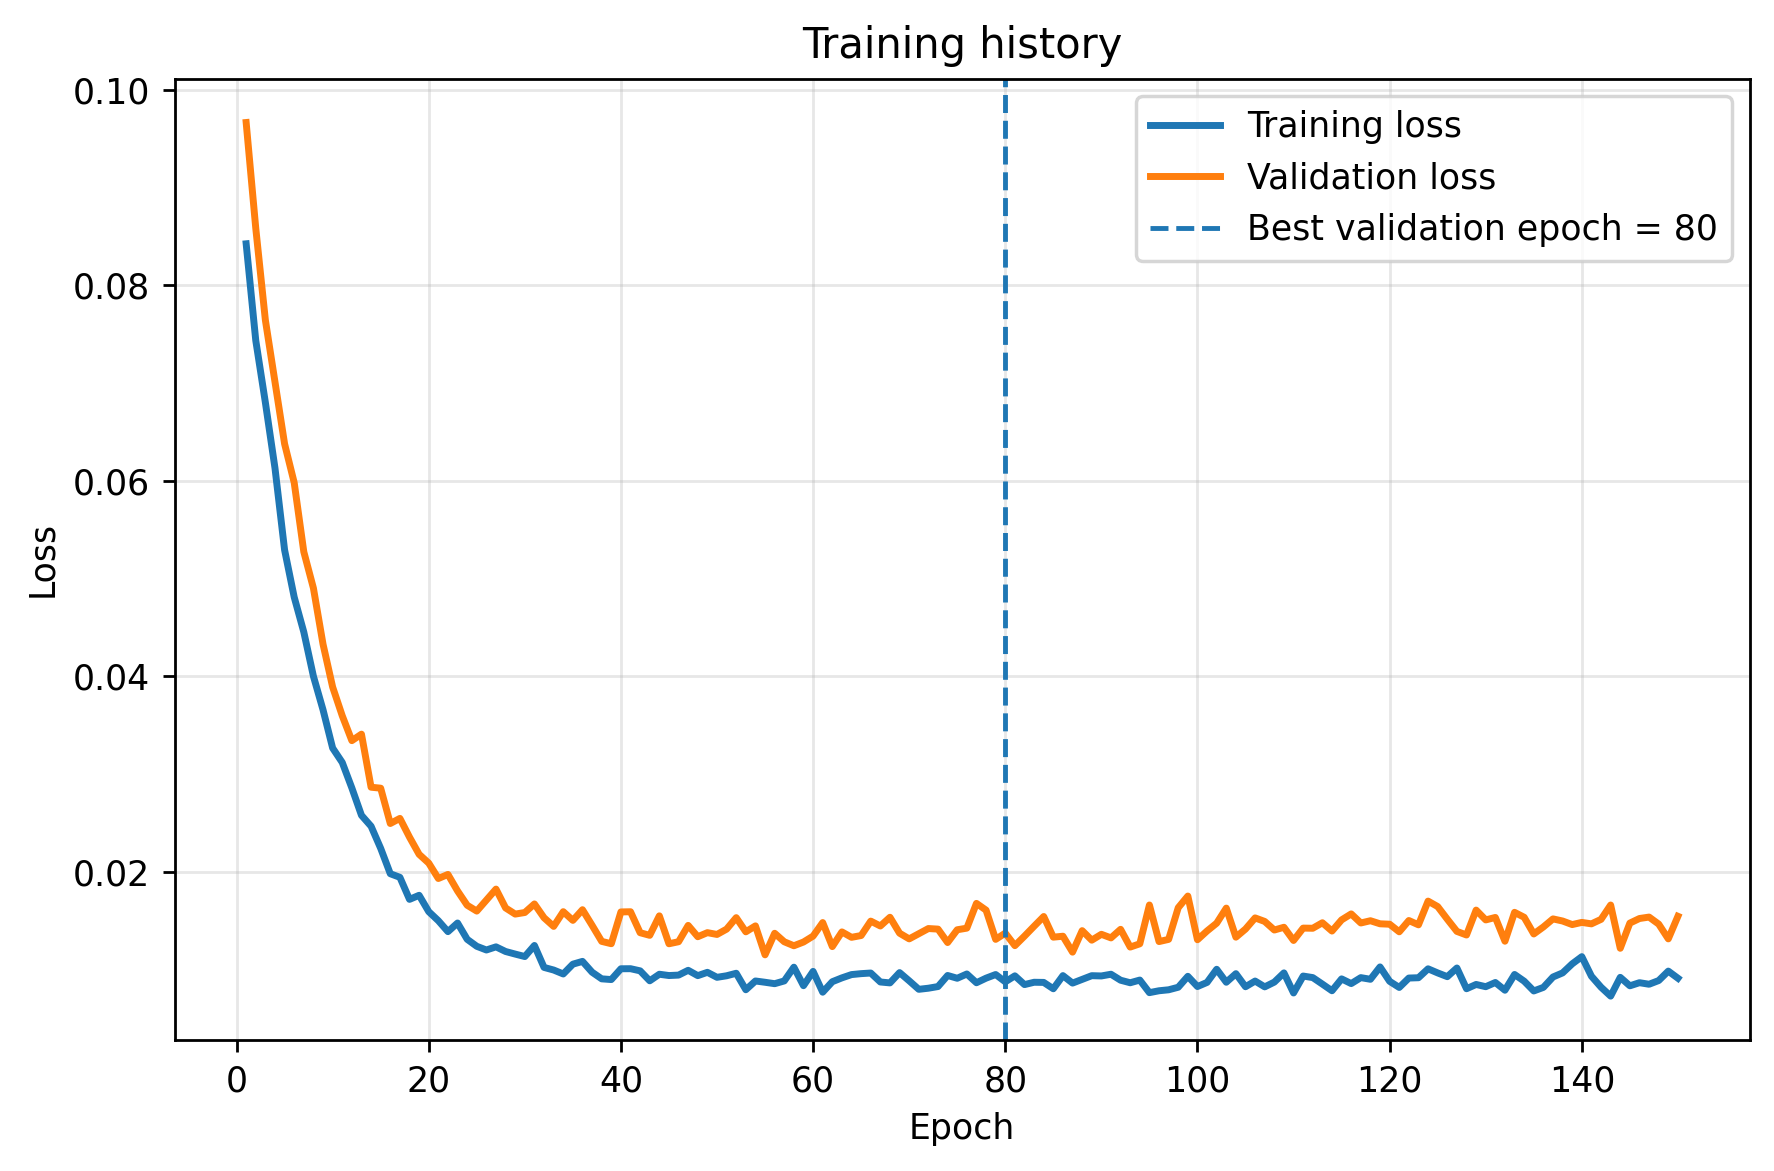
\includegraphics[width=0.82\textwidth]{images/results/png/training_history_1d.png}
    \caption{Training and validation histories for the one-dimensional FNO. The curves document optimisation convergence but do not replace held-out physical metrics.}
    \label{fig:fno_1d_training_history}
\end{figure}

For the stationary benchmark, the target profile is related to the nonlinear Ha\"issinski fixed point. Figure~\ref{fig:fno_longitudinal_reconstruction} illustrates one reconstruction and its signed residual.

\begin{figure}[H]
    \centering
    \safeincludegraphics[width=0.78\textwidth]{images/generated/training_pycolleff.png}
    \caption{Illustrative longitudinal reconstruction. The FNO prediction $\widehat{\lambda}_{\mathrm{out}}$ is compared with the reference $\lambda_{\mathrm{out}}$ and with the signed residual $\widehat{\lambda}_{\mathrm{out}}-\lambda_{\mathrm{out}}$.}
    \label{fig:fno_longitudinal_reconstruction}
\end{figure}

\begin{figure}[H]
    \centering
    \safeincludegraphics[width=0.88\textwidth]{images/generated/line_pred_truth_xsuite.png}
    \caption{Second illustrative FNO prediction. A perturbation was applied in the plotting experiment; because no multi-level, repeated-noise study was retained, this figure is not interpreted as evidence of robustness.}
    \label{fig:fno_profile_predictions_revised}
\end{figure}

No final table containing test-set $R^2$, centroid error, bunch-length error, Wasserstein distance, and inference time was exported for this preliminary block. The report therefore limits the FNO conclusion to feasibility and does not quantitatively rank it against the six-dimensional models. A robust longitudinal claim requires regeneration of these metrics using the final held-out protocol.

\subsection{CVAE snapshot reconstruction}
\label{subsec:results_latent_representation}

The next block evaluates compression and reconstruction of the fifteen pairwise marginals. Figure~\ref{fig:cvae_reconstruction_quality} shows reference, reconstruction, and residual structure for selected test states. The examples are illustrative; aggregate conclusions are based on Table~\ref{tab:cvae_reconstruction_metrics}, not on visual selection.

\begin{figure}[p]
    \centering
    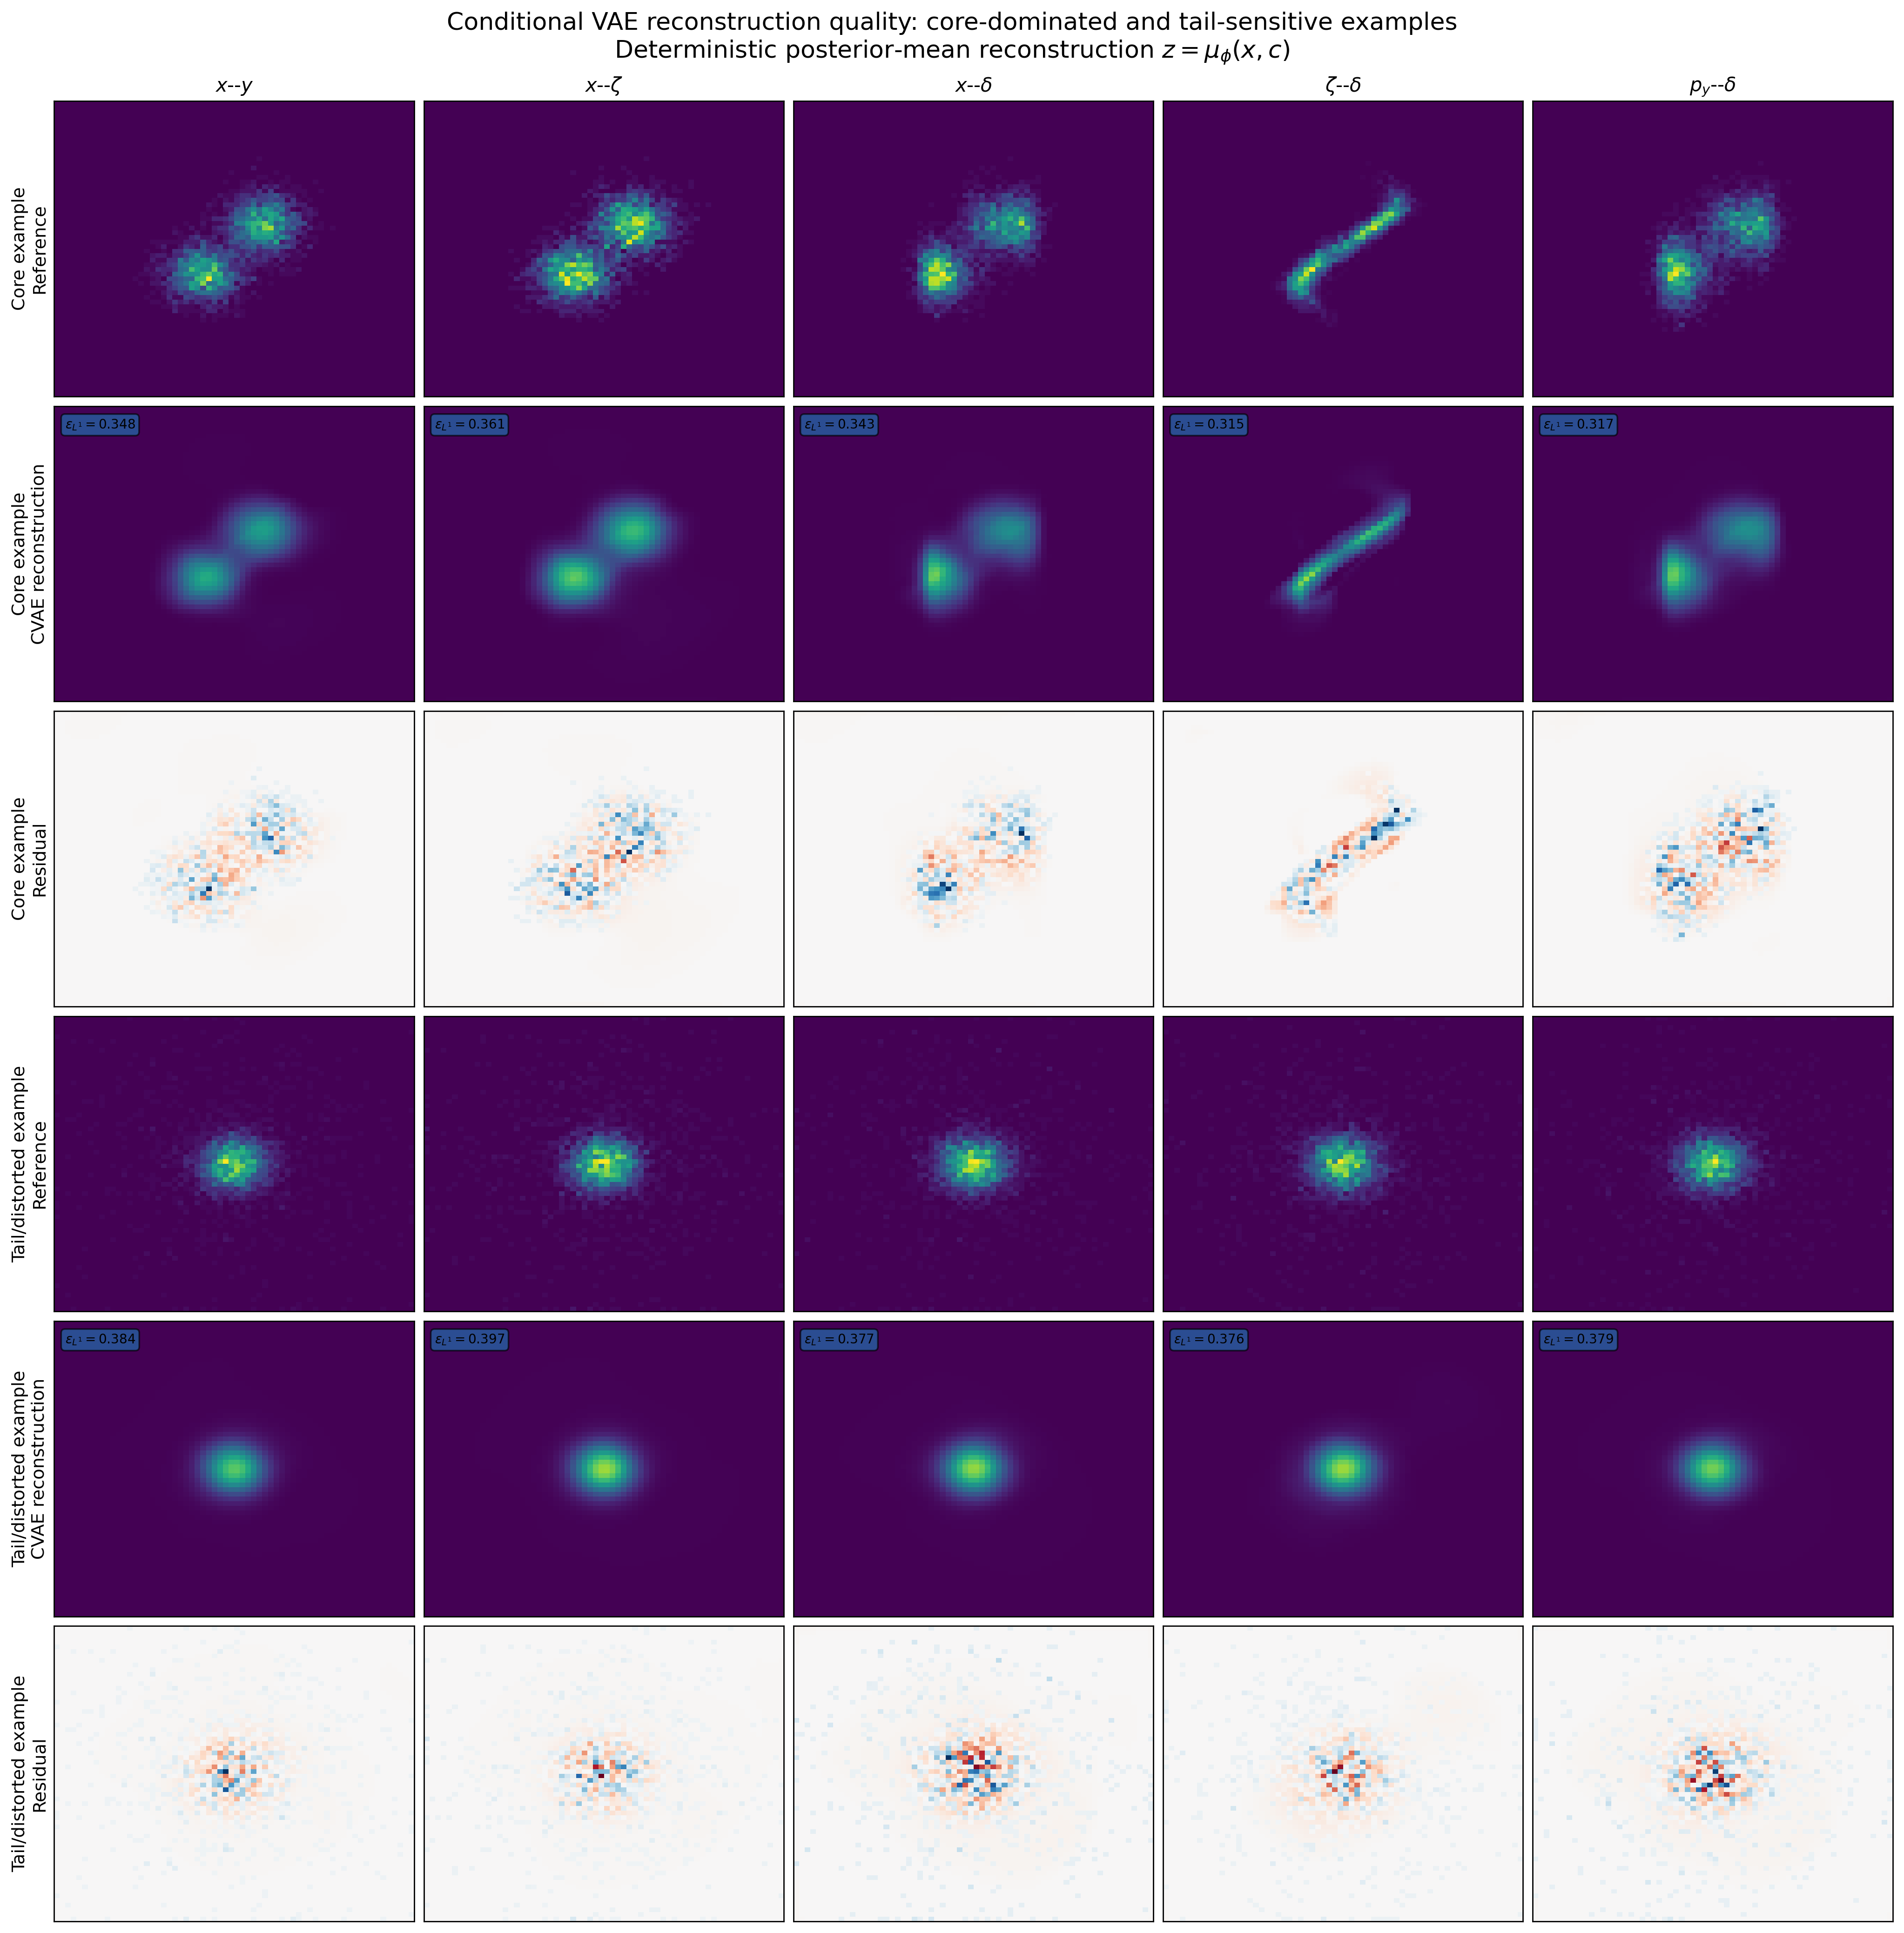
\includegraphics[width=0.96\textwidth]{images/results/png/cvae_reconstruction_quality.png}
    \caption{CVAE reconstruction quality for selected beam states. High-density cores are generally reconstructed more faithfully than low-density tails and distorted structures. Because the complete fifteen-plane panel is visually dense, individual planes should be inspected together with the aggregate test metrics.}
    \label{fig:cvae_reconstruction_quality}
\end{figure}

\begin{table}[H]
    \centering
    \caption{CVAE reconstruction metrics. The KL total is the sum over 512 latent coordinates; the per-coordinate and weighted test values are included to make its scale interpretable.}
    \label{tab:cvae_reconstruction_metrics}
    \begin{tabular}{lccc}
        \toprule
        Metric & Train & Validation & Test \\
        \midrule
        Relative histogram error & 0.362 & 0.357 & 0.367 \\
        Moment error & 0.178 & 0.243 & 0.264 \\
        KL total & 929.275 & 921.513 & 920.925 \\
        KL per latent coordinate & 1.815 & 1.800 & 1.799 \\
        Weighted KL, $\beta\mathcal{L}_{\mathrm{KL}}$ & 9.293 & 9.215 & 9.209 \\
        Sliced-Wasserstein distance & 0.0092 & 0.0089 & 0.0096 \\
        \bottomrule
    \end{tabular}
\end{table}

The similarity of train, validation, and test histogram errors provides no evidence of a large generalisation gap for this split. However, a relative histogram error of $0.367$ is not negligible. The CVAE should therefore be viewed as a lossy representation whose downstream error contains both compression and propagation contributions.

\subsubsection{Latent--physical correlation diagnostic}
\label{subsubsec:latent_space_diagnostics}

Pearson coefficients were computed between 512 latent coordinates and the twelve supplied physical observables over $N_{\mathrm{val}}=51$ validation samples,
\begin{equation}
    r_{q,z_k}
    =
    \frac{\operatorname{Cov}(q,z_k)}{\sigma_q\sigma_{z_k}}.
    \label{eq:pearson_latent_physics}
\end{equation}
This produces 6144 simultaneous coefficients.

\begin{figure}[H]
    \centering
    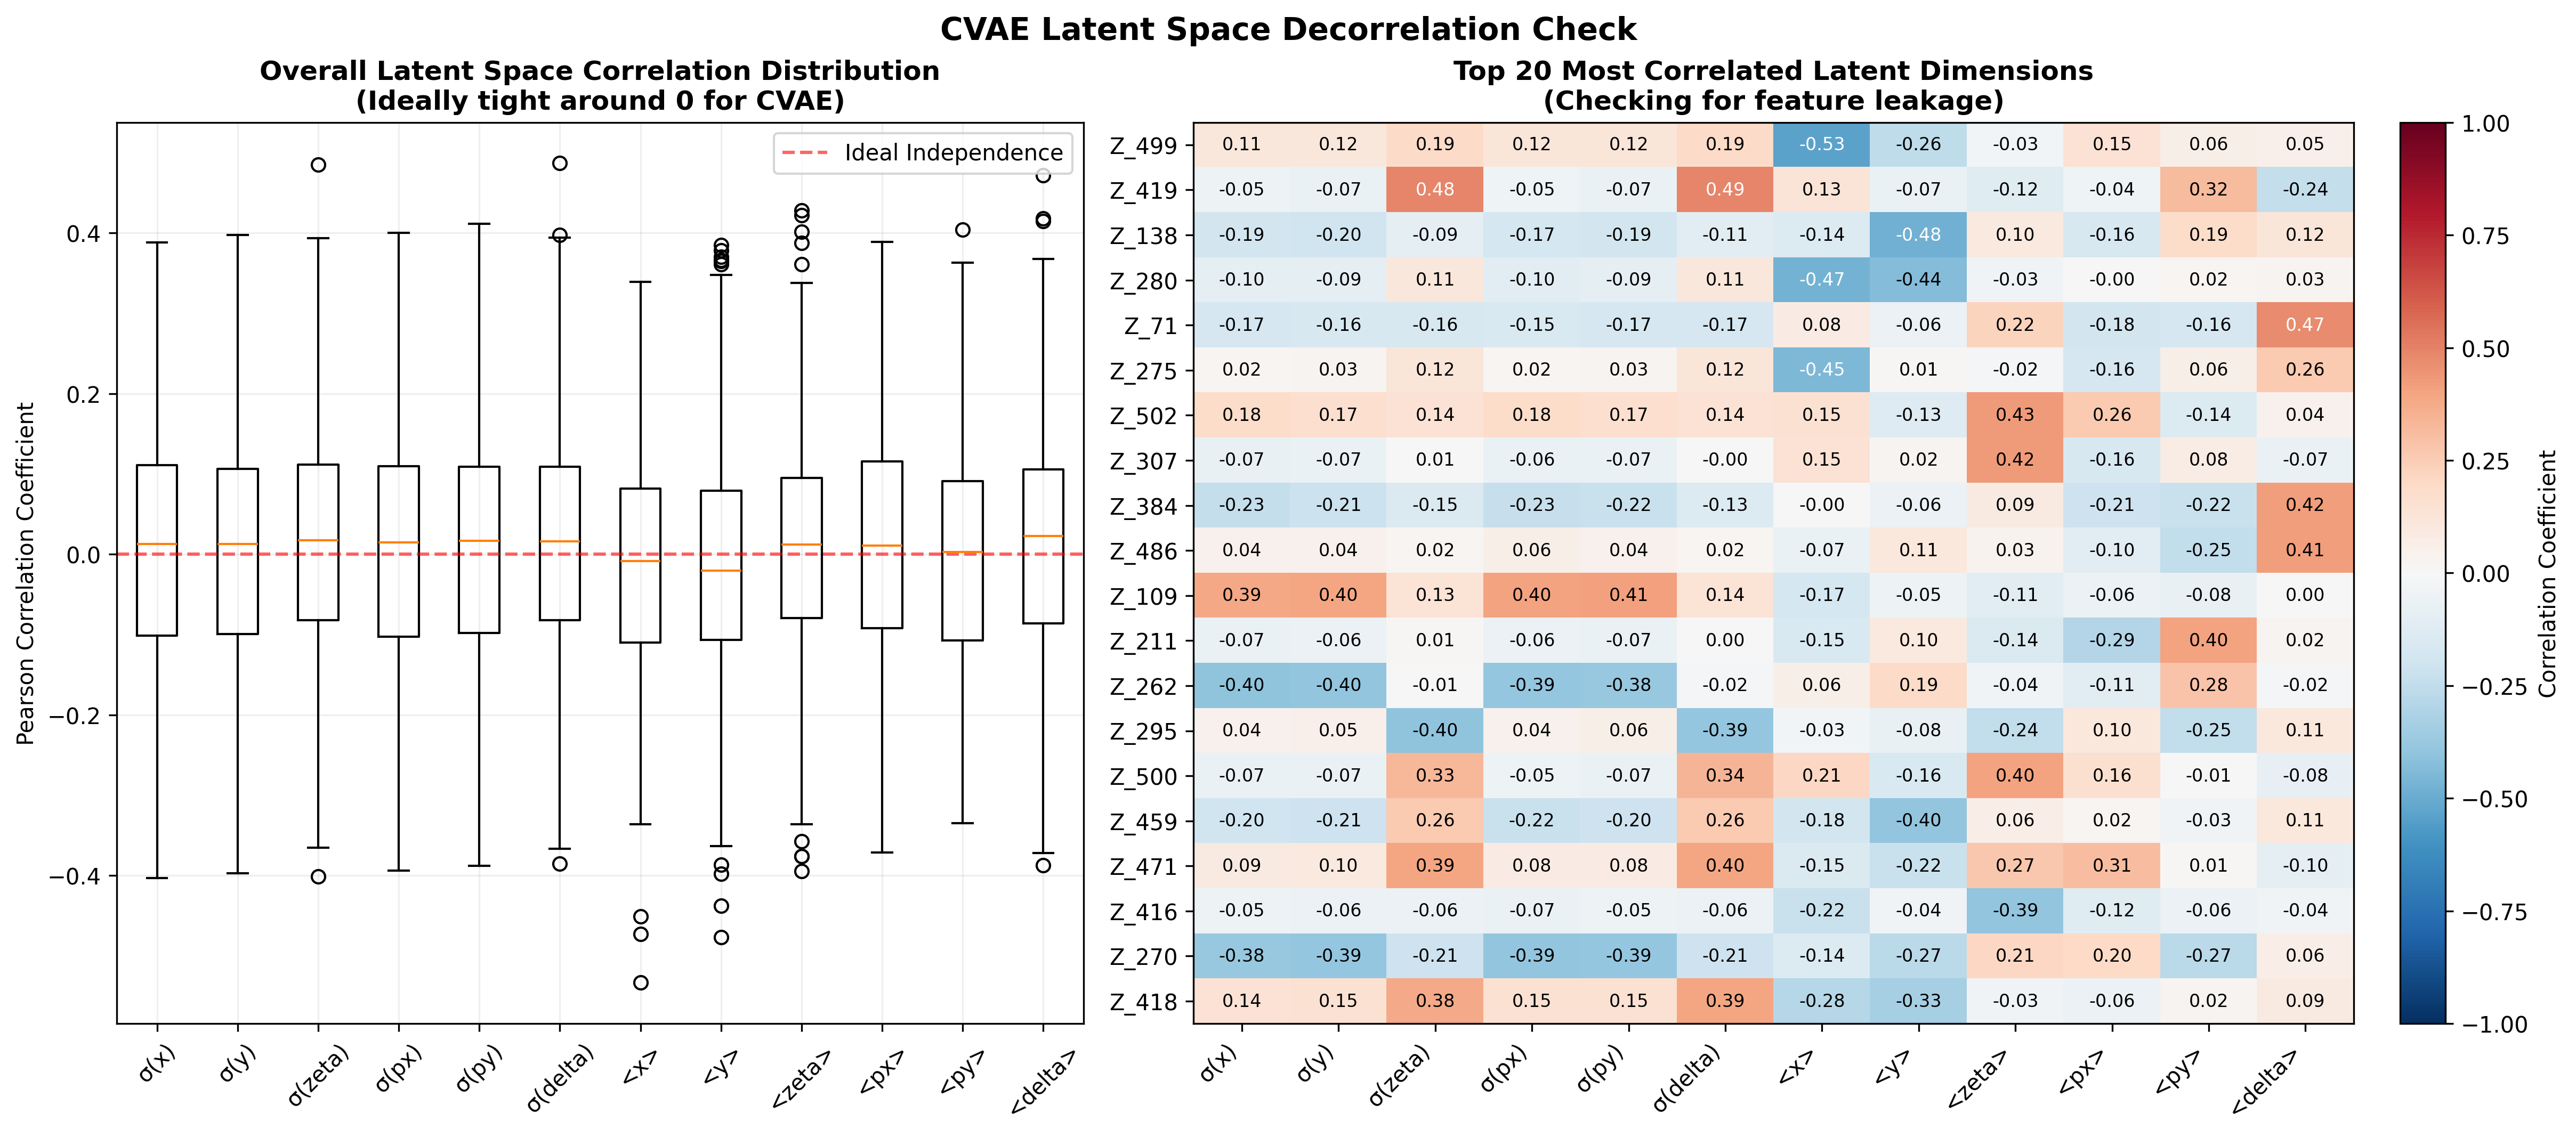
\includegraphics[width=\textwidth]{images/results/png/correlation_CVAE.png}
    \caption{Pearson correlations between the 512 latent coordinates and six RMS sizes plus six centroids. The figure is a descriptive linear-dependence diagnostic; it is not a test of latent independence or identifiability.}
    \label{fig:cvae_latent_correlation}
\end{figure}

\begin{table}[H]
    \centering
    \caption{Global latent--physical Pearson statistics on the validation subset. Threshold counts are descriptive and are not corrected significance tests.}
    \label{tab:cvae_global_correlation}
    \begin{tabular}{lcc}
        \toprule
        Diagnostic & Value & Fraction of pairs \\
        \midrule
        Mean $|r|$ & 0.1161 & -- \\
        Median $|r|$ & 0.1006 & -- \\
        Standard deviation of $|r|$ & 0.0846 & -- \\
        Maximum $|r|$ & 0.5333 & -- \\
        $|r|\geq0.30$ & 198/6144 & 3.22\% \\
        $|r|\geq0.40$ & 18/6144 & 0.29\% \\
        $|r|\geq0.50$ & 1/6144 & 0.016\% \\
        \bottomrule
    \end{tabular}
\end{table}

The observed coefficients are concentrated near zero, but the combination of $N_{\mathrm{val}}=51$ and 6144 simultaneous comparisons prevents a strong disentanglement claim. No permutation baseline, multiple-testing correction, out-of-sample linear probe, mutual-information estimate, or HSIC test was retained. The appropriate conclusion is therefore limited: the diagnostic does not reveal widespread large pairwise linear correlations, but it cannot establish statistical independence or exclude nonlinear encoding of scale and position.

\subsection{Latent propagation and conditional structure}
\label{subsec:results_transformer_locality}

\subsubsection{Global causal attention}

The global Transformer permits every token to attend to its complete upstream history. Figures~\ref{fig:tf_nowindow_marginals} and~\ref{fig:tf_nowindow_conditional_artifact} show illustrative density and conditional-mean diagnostics.

\begin{figure}[H]
    \centering
    \safeincludegraphics[width=0.94\textwidth]{images/results/png/NOWINDOW_marginals_TF.png}
    \caption{Illustrative marginal reconstructions from the global causal Transformer. Coherent residual lobes indicate systematic displacement or deformation rather than zero-centred pixel noise.}
    \label{fig:tf_nowindow_marginals}
\end{figure}

For a marginal $H(u,v)$, the conditional mean of $v$ at fixed $u$ is
\begin{equation}
    m_{v\mid u}(u)
    =
    \frac{\int vH(u,v)\,\dd v}{\int H(u,v)\,\dd v}.
    \label{eq:conditional_mean_v_given_u}
\end{equation}
This quantity probes internal dependence that may be hidden by global moments.

\begin{figure}[H]
    \centering
    \safeincludegraphics[width=0.94\textwidth]{images/results/png/artifact_nowindow_conditionals.png}
    \caption{Conditional-mean diagnostic for the global Transformer. Departures from the parity line indicate local phase-space dependence that is not reproduced by the prediction.}
    \label{fig:tf_nowindow_conditional_artifact}
\end{figure}

For reference marginal $H_{p}^{(s)}$ and prediction $\widehat{H}_{p}^{(s)}$, the signed residual is
\begin{equation}
    \varepsilon_{p}^{(s)}(u,v)
    =
    \widehat{H}_{p}^{(s)}(u,v)-H_{p}^{(s)}(u,v).
\end{equation}
Its test-set mean contributes to the bias norm $B_H$ of Eq.~\eqref{eq:histogram_bias_metric}. These diagnostics motivate the restricted-support comparison, but they do not by themselves identify global attention as the unique cause of the residuals.

\subsubsection{Windowed attention and GNO}

The same longitudinal conditional diagnostic is applied to the $W=8$ Transformer and the GNO for pair $p=11$, corresponding to $(\zeta,\delta)$ under Eq.~\eqref{eq:pair_index_order}.

\begin{figure}[H]
    \centering
    \safeincludegraphics[width=0.94\textwidth]{images/results/png/TF_conditionals_longitudinal.png}
    \caption{Conditional-slice consistency of the $W=8$ Transformer for the longitudinal $(\zeta,\delta)$ marginal. Error bars encode the local conditional spread.}
    \label{fig:tf_conditionals_longitudinal}
\end{figure}

\begin{figure}[H]
    \centering
    \safeincludegraphics[width=0.94\textwidth]{images/results/png/GNO_conditionals_longitudinal.png}
    \caption{Conditional-slice consistency of the CVAE--GNO surrogate for the longitudinal $(\zeta,\delta)$ marginal. Comparison with Fig.~\ref{fig:tf_conditionals_longitudinal} is descriptive; aggregate ranking uses Table~\ref{tab:global_model_comparison}.}
    \label{fig:gno_conditionals_longitudinal}
\end{figure}

The restricted-support models improve several aggregate metrics relative to global attention, but this comparison does not isolate locality in the strict causal sense because the configurations were independently optimised and not repeated across matched random seeds.

\subsection{Selected marginal comparisons}
\label{subsec:results_tf_gno_comparison}

Four planes from test sample $s=3$ are used as qualitative examples:
\begin{equation}
    p\in\{0,1,4,11\}
    \quad\Longleftrightarrow\quad
    (x,y),\ (x,\zeta),\ (x,\delta),\ (\zeta,\delta).
    \label{eq:selected_pair_indices_results}
\end{equation}
The sample is not used to rank the models and should not be interpreted as a statistically representative median case. It illustrates how the aggregate errors appear in concrete projected densities.

\begin{figure}[p]
    \centering
    \safeincludegraphics[width=0.96\textwidth]{images/results/png/comparison_s3_p0_x_y.png}
    \vspace{0.7em}
    \safeincludegraphics[width=0.96\textwidth]{images/results/png/comparison_s3_p1_x_zeta.png}
    \caption{Density-level comparison for illustrative sample $s=3$. Top: $(x,y)$, $p=0$. Bottom: $(x,\zeta)$, $p=1$. Each row contains the reference, $W=8$ Transformer, GNO, and signed residual maps.}
    \label{fig:tf_gno_comparison_xy_xzeta}
\end{figure}

\begin{figure}[p]
    \centering
    \safeincludegraphics[width=0.96\textwidth]{images/results/png/comparison_s3_p4_x_delta.png}
    \vspace{0.7em}
    \safeincludegraphics[width=0.96\textwidth]{images/results/png/comparison_s3_p11_zeta_delta.png}
    \caption{Density-level comparison for illustrative sample $s=3$. Top: $(x,\delta)$, $p=4$. Bottom: $(\zeta,\delta)$, $p=11$.}
    \label{fig:tf_gno_comparison_xdelta_longitudinal}
\end{figure}

\subsubsection{Derived macroparticle visualisation}

The predicted two-dimensional maps are additionally sampled to produce $10^6$ synthetic coordinate pairs per plane. Fixed histogram edges determined from the training subset are used to map bins back to physical coordinates; test-target bounds are not recomputed. The resulting samples are not an independently predicted particle cloud. They contain the same information as the corresponding 2D histogram, add Monte Carlo sampling noise, and cannot be combined into a consistent six-dimensional ensemble.

\begin{figure}[p]
    \centering
    \safeincludegraphics[width=0.90\textwidth]{images/results/png/sampling_comparison_s3_p0_x_y.png}
    \vspace{0.7em}
    \safeincludegraphics[width=0.90\textwidth]{images/results/png/sampling_comparison_s3_p1_x_zeta.png}
    \caption{Derived 2D sampling visualisation for $(x,y)$ and $(x,\zeta)$ in sample $s=3$. The plots translate density-map differences into coordinate-displacement diagnostics but provide no independent six-dimensional validation.}
    \label{fig:sampling_comparison_xy_xzeta}
\end{figure}

\begin{figure}[p]
    \centering
    \safeincludegraphics[width=0.90\textwidth]{images/results/png/sampling_comparison_s3_p4_x_delta.png}
    \vspace{0.7em}
    \safeincludegraphics[width=0.90\textwidth]{images/results/png/sampling_comparison_s3_p11_zeta_delta.png}
    \caption{Derived 2D sampling visualisation for $(x,\delta)$ and $(\zeta,\delta)$ in sample $s=3$.}
    \label{fig:sampling_comparison_xdelta_longitudinal}
\end{figure}

\subsection{Window-size dependence}
\label{subsec:results_window_study}

The validation study compares causal windows $W\in\{1,2,4,8,16,32\}$. For projection $p$,
\begin{equation}
    E_p(W)
    =
    \frac{\left\|\widehat{H}_{p}^{(W)}-H_p\right\|_2}
    {\left\|H_p\right\|_2+\varepsilon},
\end{equation}
and the reported scores are the mean and maximum over the fifteen channels.

\begin{figure}[H]
    \centering
    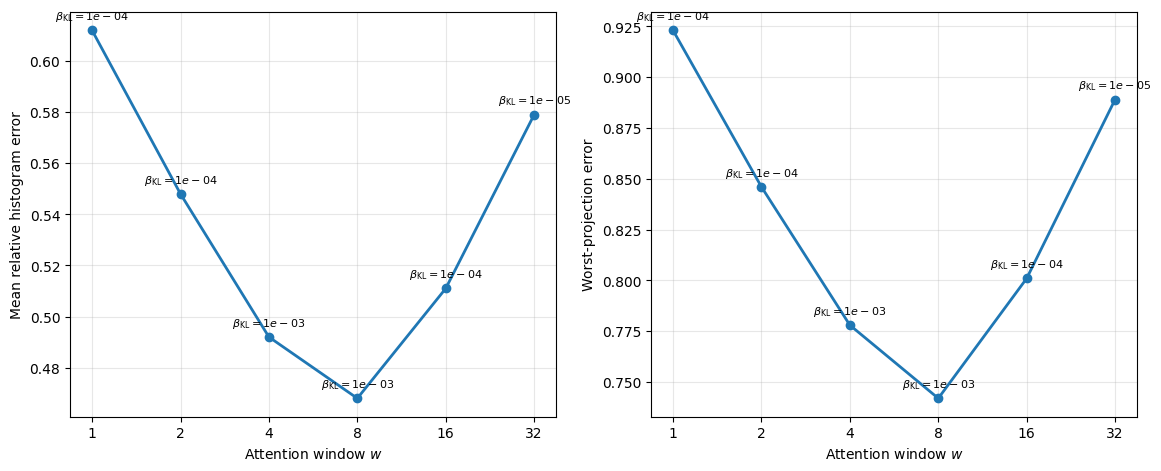
\includegraphics[width=0.98\textwidth]{images/results/png/window_results.png}
    \caption{Validation error as a function of causal window size. The KL weight was selected independently for each window, so the figure represents a tuned-model comparison rather than a fixed-regularisation ablation.}
    \label{fig:transformer_window_study}
\end{figure}

\begin{table}[H]
    \centering
    \caption{Validation-selected Transformer configurations. Each row corresponds to one selected checkpoint; uncertainty over training seeds is not available.}
    \label{tab:transformer_window_study}
    \begin{tabular}{rrrrrr}
        \toprule
        $W$ & $\beta_{\mathrm{KL}}$ & Best epoch & Mean rel. error & Worst projection & Mean KL \\
        \midrule
        1  & $1\times10^{-4}$ & 18 & 0.612 & 0.923 & 0.418 \\
        2  & $1\times10^{-4}$ & 24 & 0.548 & 0.846 & 0.356 \\
        4  & $1\times10^{-3}$ & 31 & 0.492 & 0.778 & 0.238 \\
        \textbf{8} & $\mathbf{1\times10^{-3}}$ & \textbf{34} & \textbf{0.468} & \textbf{0.742} & \textbf{0.211} \\
        16 & $1\times10^{-4}$ & 27 & 0.511 & 0.801 & 0.304 \\
        32 & $1\times10^{-5}$ & 21 & 0.579 & 0.889 & 0.447 \\
        \bottomrule
    \end{tabular}
\end{table}

The tuned validation scores are non-monotonic and attain their minimum at $W=8$. This supports the practical use of an intermediate window in the present configuration. It does not, however, prove that $W=8$ is a physical interaction length: $\beta_{\mathrm{KL}}$, checkpoint epoch, and random optimisation trajectory also vary. A stricter ablation would repeat every $W$ with fixed regularisation, matched model size, and several seeds.

\subsection{Physical-statistics prediction}
\label{subsec:results_physics_statistics}

The statistics head predicts six centroids and six RMS sizes. Figure~\ref{fig:physics_statistics_predictor} shows parity plots, while the aggregate moment errors appear in Table~\ref{tab:global_model_comparison}.

\begin{figure}[H]
    \centering
    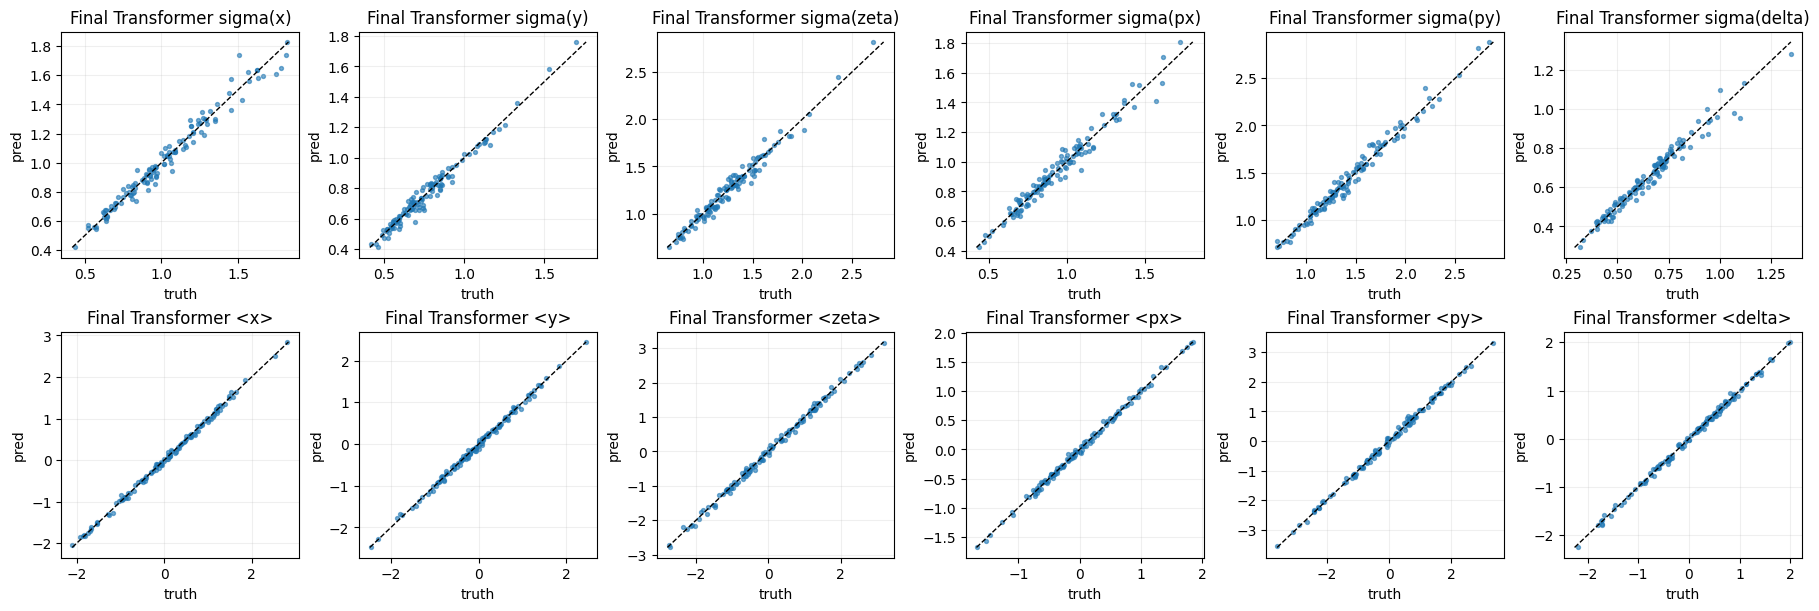
\includegraphics[width=0.95\textwidth]{images/results/png/physics_predictor.png}
    \caption{Parity plots for predicted centroids and RMS sizes across the six coordinates. The plot reveals coordinate-dependent performance; agreement in RMS size does not imply equally accurate centroids.}
    \label{fig:physics_statistics_predictor}
\end{figure}

The GNO has the lowest aggregate moment error, $0.547$, whereas the Transformer heads are substantially less accurate. In particular, the parity plots indicate that centroid prediction is more difficult than RMS-size prediction. Coordinate-wise $R_d^2$, MAE, and bias values were not retained in the exported result bundle and are therefore not invented here. Consequently, Fig.~\ref{fig:physics_statistics_predictor} supports a qualitative coordinate-wise diagnosis, while the quantitative claim is restricted to the aggregate moment errors in Table~\ref{tab:global_model_comparison}. A final rerun should export the metrics defined in Eq.~\eqref{eq:physics_r2_metric}.

\subsection{Result synthesis}

Relative to global attention, both restricted-support approaches reduce $\epsilon_{\mathrm{rel}}$ and $SW$ in the selected test checkpoints. The $W=8$ Transformer provides the lowest $SW$, while the GNO provides the best relative histogram, moment, bias, and runtime results. The data therefore support the narrower statement that structured support is beneficial for the evaluated models and split. They do not establish strict physical locality, universal architectural superiority, statistical significance across training runs, or operational validity outside the simulated parameter domain.

% =============================================================================
